
\chapter{Implementation details}
\label{implementation}

% Here we describe some of the important implementation details.



\section{Transforms}


\subsection{$N$ queens}

% [Begin Wikipedia quote] Consider a matrix with one column for each of the n ranks of the board, one column for each of the n files, and one column for each of the 4n-6 nontrivial diagonals of the board. The matrix has n^2 rows: one for each possible queen placement, and each row has a 1 in the  columns corresponding to that square's rank, file, and diagonals and a 0 in  all the other columns. Then the n queens problem is equivalent to choosing a subset of the rows of this  matrix such that every column has a 1 in precisely one of the chosen rows;  this is an exact cover problem. [end Wikipedia quote]

% Actually, the Wikipedia entry contains an error in the argumentation. On  an n by n board, we will place at most n queens. They will avoid each other by being in separate rows and columns.  But we have a total of 2n-3 parallel diagonals which have to be guarded by the n queens. Which means  that all diagonals will not be occupied. The exact cover procedure will not  find any solutions. So, in order to turn the problem into a correct exact  cover problem, we will add 4n-6 lines with a 1 only in each of the columns corresponding to the  diagonals. This will allow the algorithm to complete its search for a  complete cover by adding these rows, which we can then delete afterwards  (these will be the only rows with only a single column entry). 
% -- http://www.imtek.de/simulation//mathematica/IMSweb/imsTOC/Game%20Theory/ExactCoverDocu.html


\subsection{Polyominoes}


\subsection{Latin square}

% Application of Exact Cover to Solving the Latin Square Puzzle
% -- http://www.imtek.de/simulation//mathematica/IMSweb/imsTOC/Game%20Theory/ExactCoverDocu.html


\section{File format}

In order to store and transfer a DLX problem matrix efficiently a file format had to be defined for this specific purpose.


\subsection{Byte ordering}

Several challenges arise when defining a file format, but one of the most common is that of byte ordering.
Different platforms use different byte ordering, meaning that the order of the bytes in variables bigger than 1 byte may differ from one system to another.

Byte ordering deals with how the bytes for individual variables are ordered in memory.
For 1 byte long variables the byte ordering is irrelevant as it is only possible to order that single byte one way.
For variables longer that 1 byte the order the bytes appear in when read from and written to memory follow one of the two major conventions: big-endian or little-endian.

Big-endian stores the most significant byte (MSB) first and the least significant byte (LSB) last while little-endian does it the other way around.
In Table \ref{tab:endian} we can see that the value 0x7E, when stored in a single byte of memory, is represented in the same way for both types of byte ordering.
However, when the same value is stored in 2 bytes of memory the difference is clearly visible.


\begin{table}[htbp]
	\centering
	\begin{tabular}{|l||l|l||l|}
		\hline
		\bf Byte order & \bf 1 byte & \bf 2 byte & \bf 4 byte \\ \hline
		Big-endian    & 7E & 00 7E & 12 34 56 78 \\ \hline
		Little-endian & 7E & 7E 00 & 78 56 34 12 \\ \hline
	\end{tabular}
	\caption{Difference in representation between little and big endian when storing the value 0x7E and 0x12345678.}
	\label{tab:endian}
\end{table}

In order to achieve portability between different processor and operating system platforms one has to choose either big-endian, little-endian or a bit to indicate the byte ordering used in the file.
It is also possible to use a endian-neutral format like ASCII text or the External Data Representation (XDR) \cite{RFC4506}.

To make the file format consistent across platforms little-endian was chosen.
Following the recommendations of Intel's Endianness White Paper \cite{intel-endian} the proper byte swapping methods for big-endian systems was added.

%\cite{IEN137}
% TODO: This is where my actual decision and rationale should be stated.



\subsection{Storing sparse boolean matrices}

The storage format for the sparse boolean problem matrix has been designed for fast and efficient reading.
For libdlx to initialize its data structure it must add the nodes row by row by reading them from the left to the right side.
It starts with the top row and works its way down to the bottom just like you might read a text document.
Before the nodes are added a root node is created which is the basis for the entire structure.
To the right of the root node all the column header nodes are added in the order of increasing column indices.

\begin{algorithm}
	\caption{Create the circular doubly-linked list of columns}
	\label{alg:columns}
	\begin{algorithmic}[1]
		\STATE $R \leftarrow$ new column object
		\STATE $T \leftarrow R$
		\FOR{$i \leftarrow 1$ to the value of the $numcols$ field}
			\STATE $C \leftarrow$ new column object with index $i$
			\IF{column $i$ is a primary column}
				\STATE $C.left \leftarrow T$
				\STATE $T.right \leftarrow C$
			\ENDIF
			\STATE $T \leftarrow C$
			\STATE $H[i] \leftarrow C$
		\ENDFOR
		\STATE $R.left \leftarrow T$
		\STATE $T.right \leftarrow R$
	\end{algorithmic}
\end{algorithm}

\begin{algorithm}
	\caption{Create the circular quad-linked node structure}
	\label{alg:nodes}
	\begin{distribalgo}[1]
		\FOR{$j \leftarrow 1$ to the value of the $numrows$ field}
			\FOREACH{column index $c$ in row $j$}
				\STATE $N \leftarrow$ new node object with row index $j$
				\STATE $C \leftarrow H[c]$
				\STATE $N.column \leftarrow C$
				\STATE $C.size \leftarrow C.size + 1$
				\STATE $N.up \leftarrow C.up$
				\STATE $N.down \leftarrow C$
				\STATE $C.up.down \leftarrow N$
				\STATE $C.up \leftarrow N$
				\IF{$T$ is not set}
					\STATE $T \leftarrow N$  \COMMENT{First node in a row}
					\STATE $N.left \leftarrow N$
					\STATE $N.right \leftarrow N$
				\ELSE
					\STATE $N.left \leftarrow T$
					\STATE $N.right \leftarrow T.right$
					\STATE $T.right.left \leftarrow N$
					\STATE $T.right \leftarrow N$
				\ENDIF
			\ENDFOR
			\STATE Unset $T$
		\ENDFOR
	\end{distribalgo}
\end{algorithm}

%Challenges:
%- Format version
%- Storage of the boolean matrix (for efficient operation we first need to find out how the circular quad linked list of objects are most efficiently built. From top-left to bottom-right.


\begin{table}[htbp]
	\centering
	\begin{tabular}{|r|r|l|p{2.7in}|}
		\hline
		\bf Offset & \bf Length & \bf Field & \bf Description \\ \hline
		0  & 4 & fileid & File type ID: ``DECS'' \\ \hline
		4  & 1 & version & File format version. \\ \hline
		5  & 1 & compat & Lowest possible compatible file format version. \\ \hline
		6  & 2 & & Reserved. \\ \hline
		8  & 4 & numcols & Number of columns $> 1$. \\ \hline
		12 & 4 & numrows & Number of rows $> 1$. \\ \hline
		16 & 4 & numelems & Number of non-zero values in the matrix $> 1$. \\ \hline
		20 & 4 & elements & Byte offset to the matrix element entries. Should never be 0. \\ \hline
		24 & 4 & names & Byte offset to the column and row name list. 0 if unavailable. \\ \hline
		28 & 4 & probid & Problem type ID. Each problem type has a unique ID so that the correct transform can be chosen and the problem specific information can be decoded. \\ \hline
		32 & 4 & probinfo & Byte offset to problem specific information. 0 if unavailable. \\ \hline
		36 & 4 & blind & Byte offset to problem specific information. 0 if unavailable. \\ \hline
%		26 & 2 & Number & Job ID. Each problem type has a unique ID so that the correct transform is selected. \\ \hline
	\end{tabular}
	\caption{File header format. Offset and length in bytes.}
	\label{tab:header}
\end{table}

The file header format is made as simple as possible to allow future extensions to be made without breaking backwards compatibility.
The compat field indicates the lowest possible file format version implemented which will be able to read this version of the file.
This means that if the file format version implemented in a program is lower than the compat field it will not be able to read and process it correctly.

\begin{figure}[htb]
	\centering
	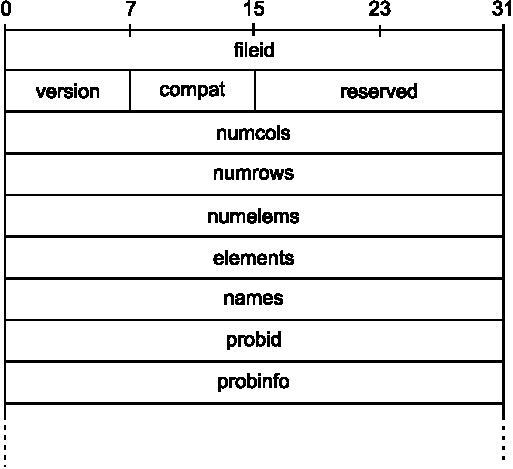
\includegraphics[width=0.6\textwidth]{headerformat.pdf}
	\caption{File header format structure}
	\label{fig:header}
\end{figure}


The DLX algorithm itself does not use the column and row names or the problem type ID and the problem specific information.
This information can be used by the BOINC client to display graphical information during the computation.
For example it can use the problem type ID to identify the correct transform, and when the DLX algorithm finds a solution it can run the reverse transform and display the solution graphically.
BOINC has built-in support for OpenGL rendering and the solution can be displayed as part of a special BOINC screen saver.

\subsubsection{Bit packing}

If we allow the number of bits used to store the column and row numbers to be an arbitrary integer (instead of 8, 16 or 32) we can achieve a reduction in file size without too much additional work.
By applying a technique known as bit packing, a form of lossless compression, we can exploit the otherwise unused bits.
As long as we know the range of our values, as we do with the numcols and numrows fields, we can easily apply this technique.
In the May 2002 edition of Game Developer Magazine Jonathan Blow wrote, in The Inner Product column, about how bit packing can be implemented \cite{gdip_bitpack}.
He also explained a generalization of the bit packing scheme which packs the data even more densely by doing sub-bit precision packing.
For the sake of simplicity sub-bit precision packing will not be implemented at this time.
The ``Bit Packing: A Network Compression Technique'' article \cite{gpg_bitpack} by Pete Isensee in Game Programming Gems 4 gives a framework for implementing bit packing in C/C++.
Other techniques for lossless compression 

By using bit packing we incur an extra processing overhead when reading and writing the file as the program will have to apply some bit shifting and modulus operations to retrieve the actual values.
The trade off between processing overhead and file size can be beneficial in cases where the number of non-zero elements, rows and/or columns is large and where storage and bandwidth resources are scarce.
A bit packing framework will need to determine how many bits are required to accommodate the values of the colnum and rownum fields.
For column and row indexes starting at 1 this means that $B \geq 1 + \log_2{n}$, where $B$ is the number of bits used to store the indexes and $n$ is the total number of row or columns.
Optimal bit packing is achieved when $B = 1 + \lfloor \log_2{n} \rfloor$, but for the non-conventional sub-bit precision packing this will be sub optimal unless $B = 1 + \log_2{n}$.

In the following description of the 


\begin{table}[htbp]
	\centering
	\begin{tabular}{|r|r|l|p{2.7in}|}
		\hline
		\bf Offset & \bf Length & \bf Field & \bf Description \\ \hline
		0     & $B_c$ & colnames & Number of column names \\ \hline
		$B_c$ & 4     &  & Number of column names \\ \hline
		4     & 4     &   & Byte offset to problem specific information. 0 if unavailable. \\ \hline
	\end{tabular}
	\caption{File format for column and row names}
	\label{tab:colrowformat}
\end{table}





\section{libdecs}


%\subsection{Modes of operation}

% TODO: Fix this if we are able to return only the row numbers from the computing nodes (the DLX library).
%DECS has two basic modes of operation regarding how it handles the return values of the system.
%In the first mode, which is the most common, the system will store and forward all the solutions it finds back to the DECS server.
%This provides the calling application with the full set of solutions so that it can run a detailed analysis on them or save them for later use.
%For problems which generates a very large number of solutions or solutions this approach can cause a huge strain on the system.
%The storage and bandwidth capacities of the computing nodes and the DECS server could cause considerable delays.
%In extreme cases it might even cause some or all of the solutions to never be returned.

%A policy of not accepting overly large problem matrices could be implemented to prevent this problem.
%This works well because the memory requirements of the DLX algorithm is proportional to the size of the problem matrix.
%However, it does not do us much good because the problem will remain unsolved.

%The second mode of operation will simply discard the solution matrices, but it keeps a count on the number of solutions
%It will only keep a count

%A possible extension to this would be to add other return values than number of solutions.
%Each solution the DLX algorithm arrives at could be further analyzed so that other aspects of the solutions could be returned.



\section{BOINC}

\subsection{Architecture}


\section{libdlx}

The main purpose of libdlx is to parse a file with the problem matrix and to apply the DLX algorithm in order to solve it.
The theory behind the DLX algorithm has been covered in Chapter \ref{dancing_links}.
Here we will look at the external interface to libdlx and some of its internals.

% Challenges
% - Node and column objects. How to find the correct row number to reduce data sent back to the server.
% - Building the boolean matrix

\subsection{Building the boolean matrix}
\label{matrix_construction}

Before the DLX algorithm can be started the matrix needs to be read from a file and the data structures must be initialized.
In the case of libdlx each non-zero element in the matrix is a quad-linked node in a circular quad-linked structure.
To actually construct this data structure we need some column objects as well.

% TODO: Add pseudocode for matrix creation.